\documentclass[11pt, reqno]{amsart} \usepackage{hyperlatex}
\usepackage{graphicx} \usepackage{amsmath} \usepackage{hyperref}
\usepackage{amssymb,amsxtra,amsthm,amscd}
\begin{document}

\htmltitle{An introduction to multiple linear regression}
\htmladdress{data supermodels} \title[Multiple regression]{An
  introduction to \\ multiple linear regression} \author{Anthony
  D.~Blaom}
\maketitle
\tableofcontents

\section*{Simple linear regression and its limitations}
Suppose you are a credit provider wanting to predict the expected
annual returns for prospective customers, based on a history of
previous customers. By ``annual returns'' we mean interest collected
less any defaulting amount or collection costs, divided by the total
number of years your company provided credit. For illustrative purposes, we
suppose that this history consists of the salary and the debt, at the
time of credit application, for fifteen customers whose annual returns
are known; new customers are to provide their current salary and debt
as part of their application. Scatterplots of the historical data are
shown in Figures \ref{fig:1} and \ref{fig:2}.

\begin{figure}[h]
  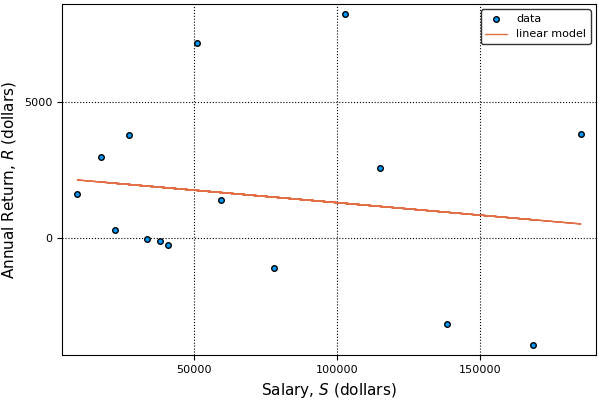
\includegraphics[scale=0.6]{model1.png}
  \caption{Scatterplot of annual return versus salary,
    fitted with a straight line minimising the summed squared error.}
  \label{fig:1}
\end{figure}

\begin{figure}
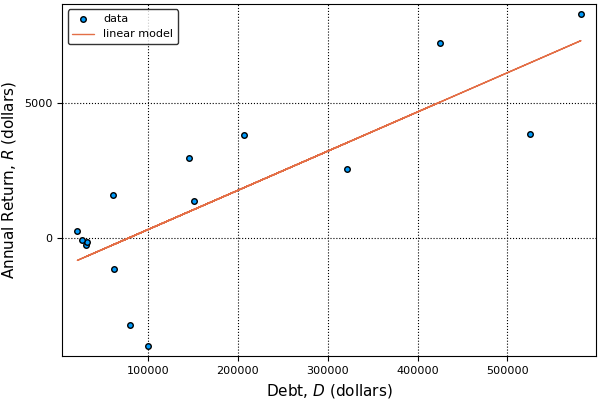
\includegraphics[scale=0.6]{model2.png}
\caption{Scatterplot of annual return versus debt, fitted with a
  straight line minimising the summed squared error.}
      \label{fig:2}
\end{figure}

You are familiar with simple linear regression, a technique for
fitting a ``line of best fit'' to two-dimensional data, and have done
so for: (i) the annual return $R$, as a function of the salary $S$;
and (ii) $R$ as a function of the debt $D$. Equations describing the
fitted lines (also shown in the figures) are:
\begin{align*}
  R &= 2\,220 - 0.0092 S, \\
  R &= -1\,120 + 0.014 D. 
\end{align*}
It is not immediately clear to you how to combine these two linear
models into a {\em single} equation for $R$. However, after some
thought, you try for a linear equation in {\em two} variables, i.e.,
one of the form
\begin{equation}
  \label{eq:1}
  R = b + w_1 S  + w_2 D,
\end{equation}
where $b,w_1,w_2$ are constants. Furthermore, you argue that the
``weights'' $w_1$ and $w_2$ ought to come from the simple linear
models already obtained --- i.e., $w_1 = -0.0092$ and $w_2=0.014$ ---
and decide to choose the ``bias'' $b$ by requiring that combined model
predicts the {\em mean} return $\bar R$ when mean values for $S$ and
debt $D$ are substituted:
\begin{align*}
  \bar R &= b + w_1 {\bar S} + w_2 {\bar D},\\
  \text{which gives}\quad b &= {\bar R} + 0.0092 {\bar S} - 0.014
  {\bar D}.
\end{align*}
After computing the mean values from the historical data, this gives
you $b= -270$, and a final model,
\begin{equation}
  \label{eq:2}
  R = -270 -0.0092 S + 0.014 D.
\end{equation}

Before rushing off to your boss with the new model, you decide you had
better check its performance. Comparing predictions of the new model
with the historical annual return data, you calculate a
root-mean-squared error of $\$1480 $. Yikes! Compared with the average
return, ${\bar R} = \$1549$, this seems quite high. 

On the other hand, you only had a small --- and obviously noisy ---
data set to work with; so perhaps this is as good as can be expected.

Just then your boss bursts into the room.

``Never mind the credit model, Bill. Jane's found a model that fits
the data perfectly. Better luck next time, hey!''

Mmmm. What went wrong?

\section*{Fitting multidimensional data: multiple regression}
Naturally, you are suspicious of claims to fit the data
perfectly. In fact the data discussed above is described perfectly by
a linear model of the form \eqref{eq:1}, but only because it was
cooked up to do just that.  However, the coefficients for the perfect
fit look quite different from those in \eqref{eq:2} above:
\begin{equation}
  R =  750 - 0.04S + 0.02D
\label{eq2}
\end{equation}
Note also that there is no ``noise'' in the annual return data at all,
only artificially generated noise in the $S$ and $D$ values for which
corresponding $R$ values were calculated using \eqref{eq2}.

The point to be made here is that simple linear regression has very
limited value when dealing with a quantity like annual returns that
depends on more than one customer attribute. The reason for
these limitations become obvious when we look at all the data {\em
  simultaneously}, i.e., in a three-dimensional plot; see Figure
\ref{fig:3}. All the data can be seen to lie on a single plane (the
plane whose defining equation is \eqref{eq2}), a fact completely
obscured in the two-dimensional projections of the data presented in
Figures \ref{fig:1} and \ref{fig:2}.
\begin{figure}
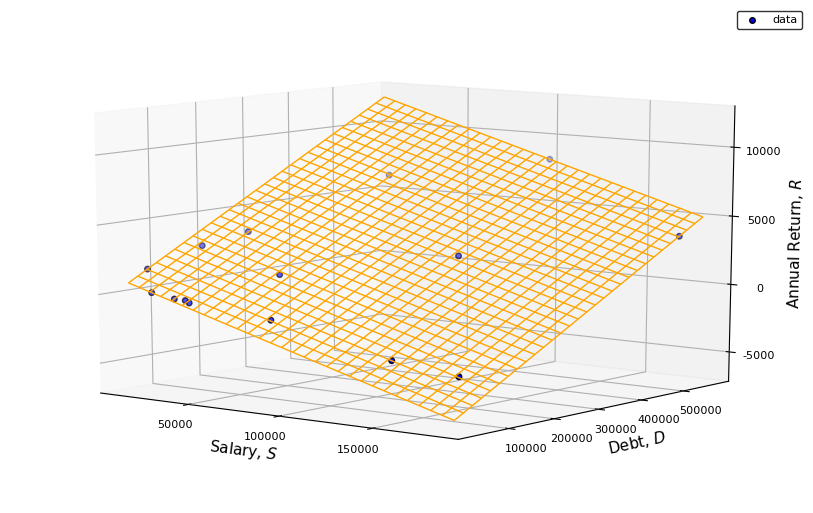
\includegraphics[scale=0.6]{model3.png}
  \caption{A three-dimensional plot of the salary, debt, annual
    return historical data, together with a plane containing all data
    points.}
  \label{fig:3}
\end{figure}

In the case of one output variable (such as $R$) and two input
variables ($S$ and $D$), multiple regression is a technique finding
the {\em plane} of best fit. If one has more than two input variables,
the technique fits a {\em hyper}\,plane to the data. In any case, the
output of the method is a formula expressing outputs as a linear
function of the inputs (plus a constant ``bias'' term).

Any statistical package will perform multiple regression; but before
using one you'll want some idea of how it works. For simplicity we
describe the method here for the three-dimensional credit scoring
problem described above. We assume a basic familiarity with matrix
algebra.

Equation \eqref{eq:1} is the general form of a plane in $S$-$D$-$R$
space. Ideally, we seek values for the unknowns $b$, $w_1$, and $w_2$
such that this equation holds for every instance of the historical
data. That is, we want
\begin{align*}
  R_1 &= b + w_1 S_1 + w_2 D_1\\
  R_2 &= b + w_1 S_2 + w_2 D_2\\
R_3 &= b + w_1 S_3+ w_2 D_3\\
\vdots & \qquad \vdots \qquad \qquad \vdots\\
R_{15} &= b + w_1 S_{15} + w_2 D_{15},
\end{align*}
where $(S_j,D_j,R_j)$ is the $j$th instance of the Salary-Debt-Annual
Return data. In general we cannot solve these equations exactly but
try to minimize the errors $e_1, e_2, \ldots, e_{15}$, defined by
\begin{align*}
  e_1 &= R_1 - b - w_1 S_1 - w_2 D_1\\
  e_2 &= R_2 - b - w_1 S_2 - w_2 D_2\\
  e_3 &= R_3 - b - w_1 S_3 - w_2 D_3\\
\vdots & \qquad \vdots \qquad \qquad \vdots\\
e_{15} &= R_{15} - b - w_1 S_{15} - w_2 D_{15},
\end{align*}
These equations defining the error may be written in matrix form,
\begin{equation*}
   {\mathbf e} = {\mathbf R} - {\mathbf X} {\mathbf w},  
\end{equation*}
where $\mathbf e$, $\mathbf R$ and $\mathbf w$ are the column vectors
defined by
\begin{equation*}
{\mathbf e} =
\begin{bmatrix}
  e_1\\
e_2\\
e_3\\
\vdots\\
e_{15}
\end{bmatrix}, \qquad 
{\mathbf R} =
\begin{bmatrix}
  R_1\\
  R_2\\
  R_3\\
  \vdots\\
  R_{15}
\end{bmatrix}, \qquad 
{\mathbf w} = 
\begin{bmatrix}
  b\\
w_1\\
w_2
\end{bmatrix},  
\end{equation*}
and ${\mathbf X}$ is the $15\times 3$ matrix given by
\begin{equation*}
  \mathbf X =
  \begin{bmatrix}
    1 & S_1 & D_1 \\
1 & S_2 & D_2 \\
1 & S_3 & D_3 \\
\vdots & \vdots & \vdots \\
1 & S_{15} & D_{15}
  \end{bmatrix}.
\end{equation*}
Now the root-mean-square error is just the length of the
15-dimensional vector ${\mathbf e} = {\mathbf R} - {\mathbf X}
{\mathbf w}$. One can show that the vector $\mathbf w$ that minimizes
this length is the one for which $({\mathbf X}\mathbf v)^{\mathsf T}
{\mathbf e} = 0$, for all $3$-dimensional row vectors ${\mathbf v}$;
here ${\mathsf T}$ denotes transpose. (In other words, $\mathbf e$
should be perpendicular to the range space of $\mathbf X$.)
Therefore, we need
\begin{equation*}
  {\mathbf v}^{\mathsf T}({\mathbf X}^{\mathsf T} {\mathbf R} -
  {\mathbf X}^{\mathsf T} {\mathbf X} {\mathbf w})=0,
\end{equation*}
for all ${\mathbf v} $. But this holds whenever the bracketed term
vanishes. Assuming the $3 \times 3$ matrix ${\mathbf X}^{\mathsf T}
{\mathbf X} $ is invertible, we deduce the following formula for the
sought after vector ${\mathbf w}$:
\begin{equation}
  {\mathbf w} = ({\mathbf X}^{\mathsf T} {\mathbf X})^{-1}{\mathbf
    X}^{\mathsf T} {\mathbf R}.
\end{equation}

The $3\times 15$ matrix
$({\mathbf X}^{\mathsf T} {\mathbf X})^{-1}{\mathbf X}^{\mathsf T}$ is
known as the {\em pseudoinverse} (or {\em left inverse}) of
${\mathbf X}$. This is what statistical packages typically calculate
to carry out multiple regression (usually by first computing the
so-called singular value decomposition of ${\mathbf X}$).

\section*{Alternative approaches} With a more sophisticated method comes new
traps and multiple regression is no exception. If, for example, two of
your customer attributes are closely correlated, then it will be
difficult for your package to accurately compute the inverse of
${\mathbf X}^{\mathsf T}{\mathbf X}$, because its determinant will be
close to zero. A solution in that case is to decorrelate the data
(drop some variables depending essentially on others). Sometimes
correlations in the data can be detected by simple pair-wise
correlation tests; otherwise a more sophisticated method, such as
principal component analysis, may be called for (although this
technique also has limitations associated with certain linearity assumptions).

There are algorithms for constructing linear models that avoid directly
computing inverses altogether. Quite popular are so-called {\sl
  regularised} linear models, such as ridge regression, the lasso, and
elastic net models. 

More significantly, the most accurate credit scoring system is
unlikely to be based on simple linear models. Large credit issuing
companies often employ sophisticated modelling techniques - artificial
neural networks, support vector machines, random forests, and gradient
boosted trees, to name a few. In fact, these models are so good that
new dangers occur, such as {\em overfitting} (fitting the noise rather
than the "underlying trend") and {\em data snooping}, topics beyond
the scope of this article.

% \section*{Doing it in Microsoft Excel}
% To perform multiple regression using an Excel spreadsheet, one can use
% the {\tt LINEST} function. Below is an Excel screenshot for the example
% above. 

% You can download the spreadsheet itself from
% \href{file:///Users/anthony/Dropbox/Math_Expertise/credit.xlsx}{here}.

% \begin{figure}[h]
%   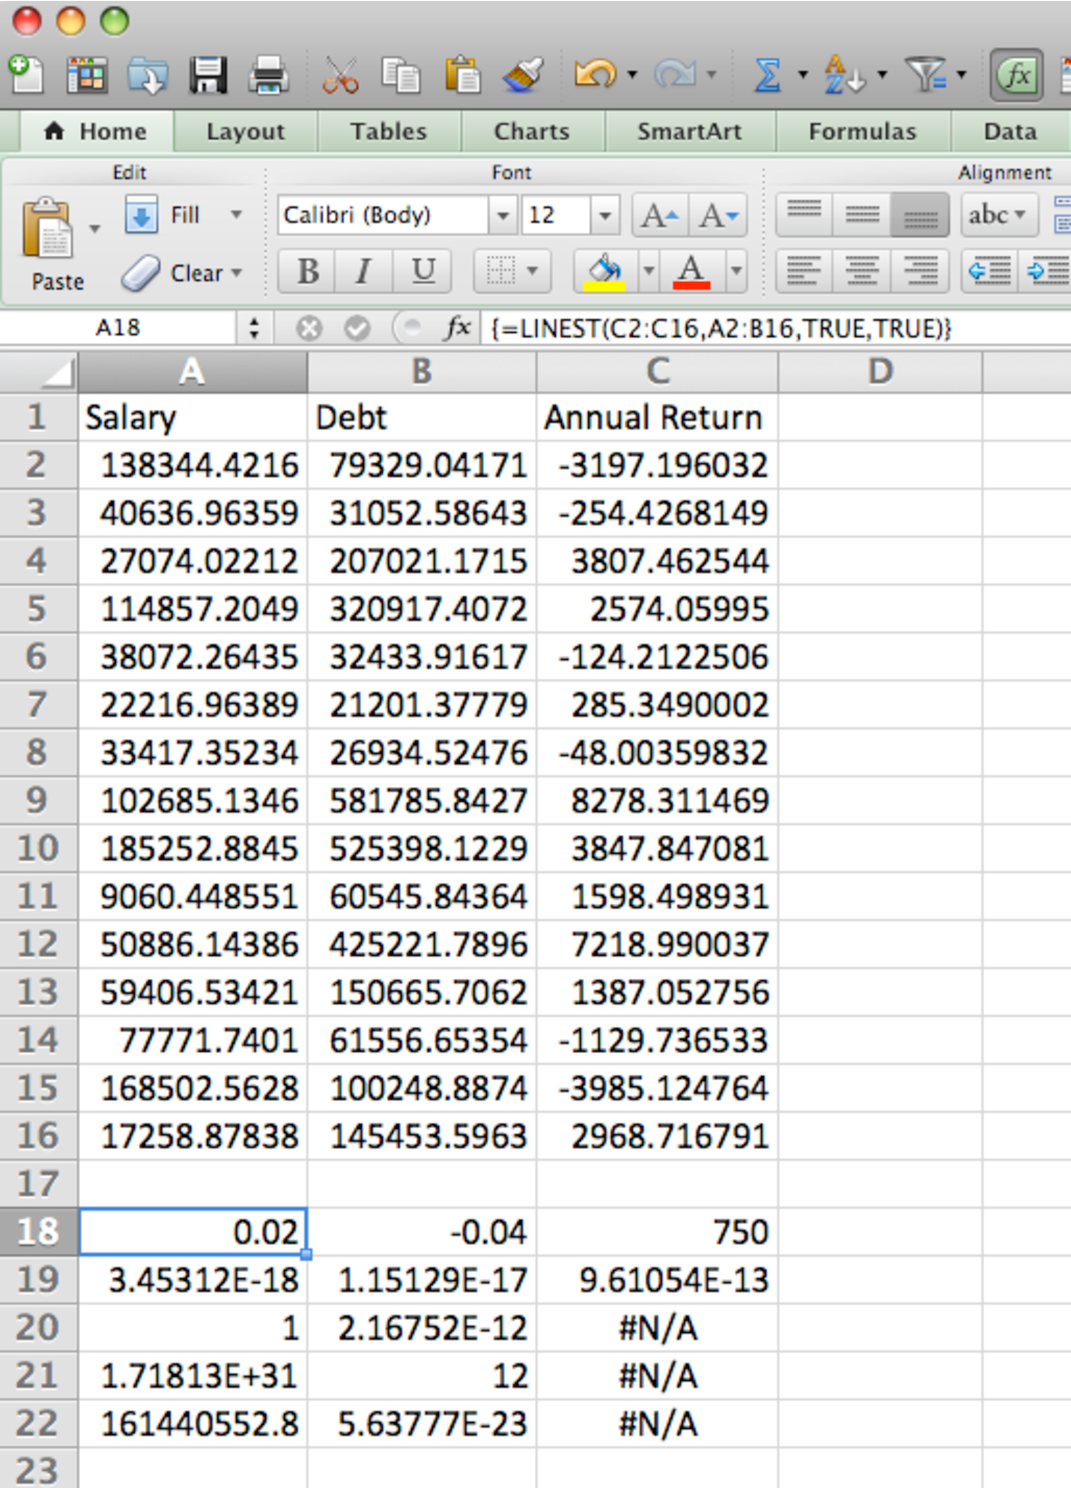
\includegraphics[scale=0.4]{excel_screen_shot.pdf}
%   \caption{Performing multiple regression using Microsoft Excel}
%   \label{fig:4}
% \end{figure}


% The figures in Row 18 show the weights $w_1$ and $w_2$ , and the bias
% $b$, as computed by the {\tt LINEST} function, which is entered in
% cell A18 (as an array formula). See Excel's built in documentation for
% details.
\vfill
\noindent%
August, 2012; this version compiled \today

\end{document}